\section{Internal documents} \label{toc:internedokumente}

\subsection{Layout Mining Data Center} \label{toc:layoutkardok}
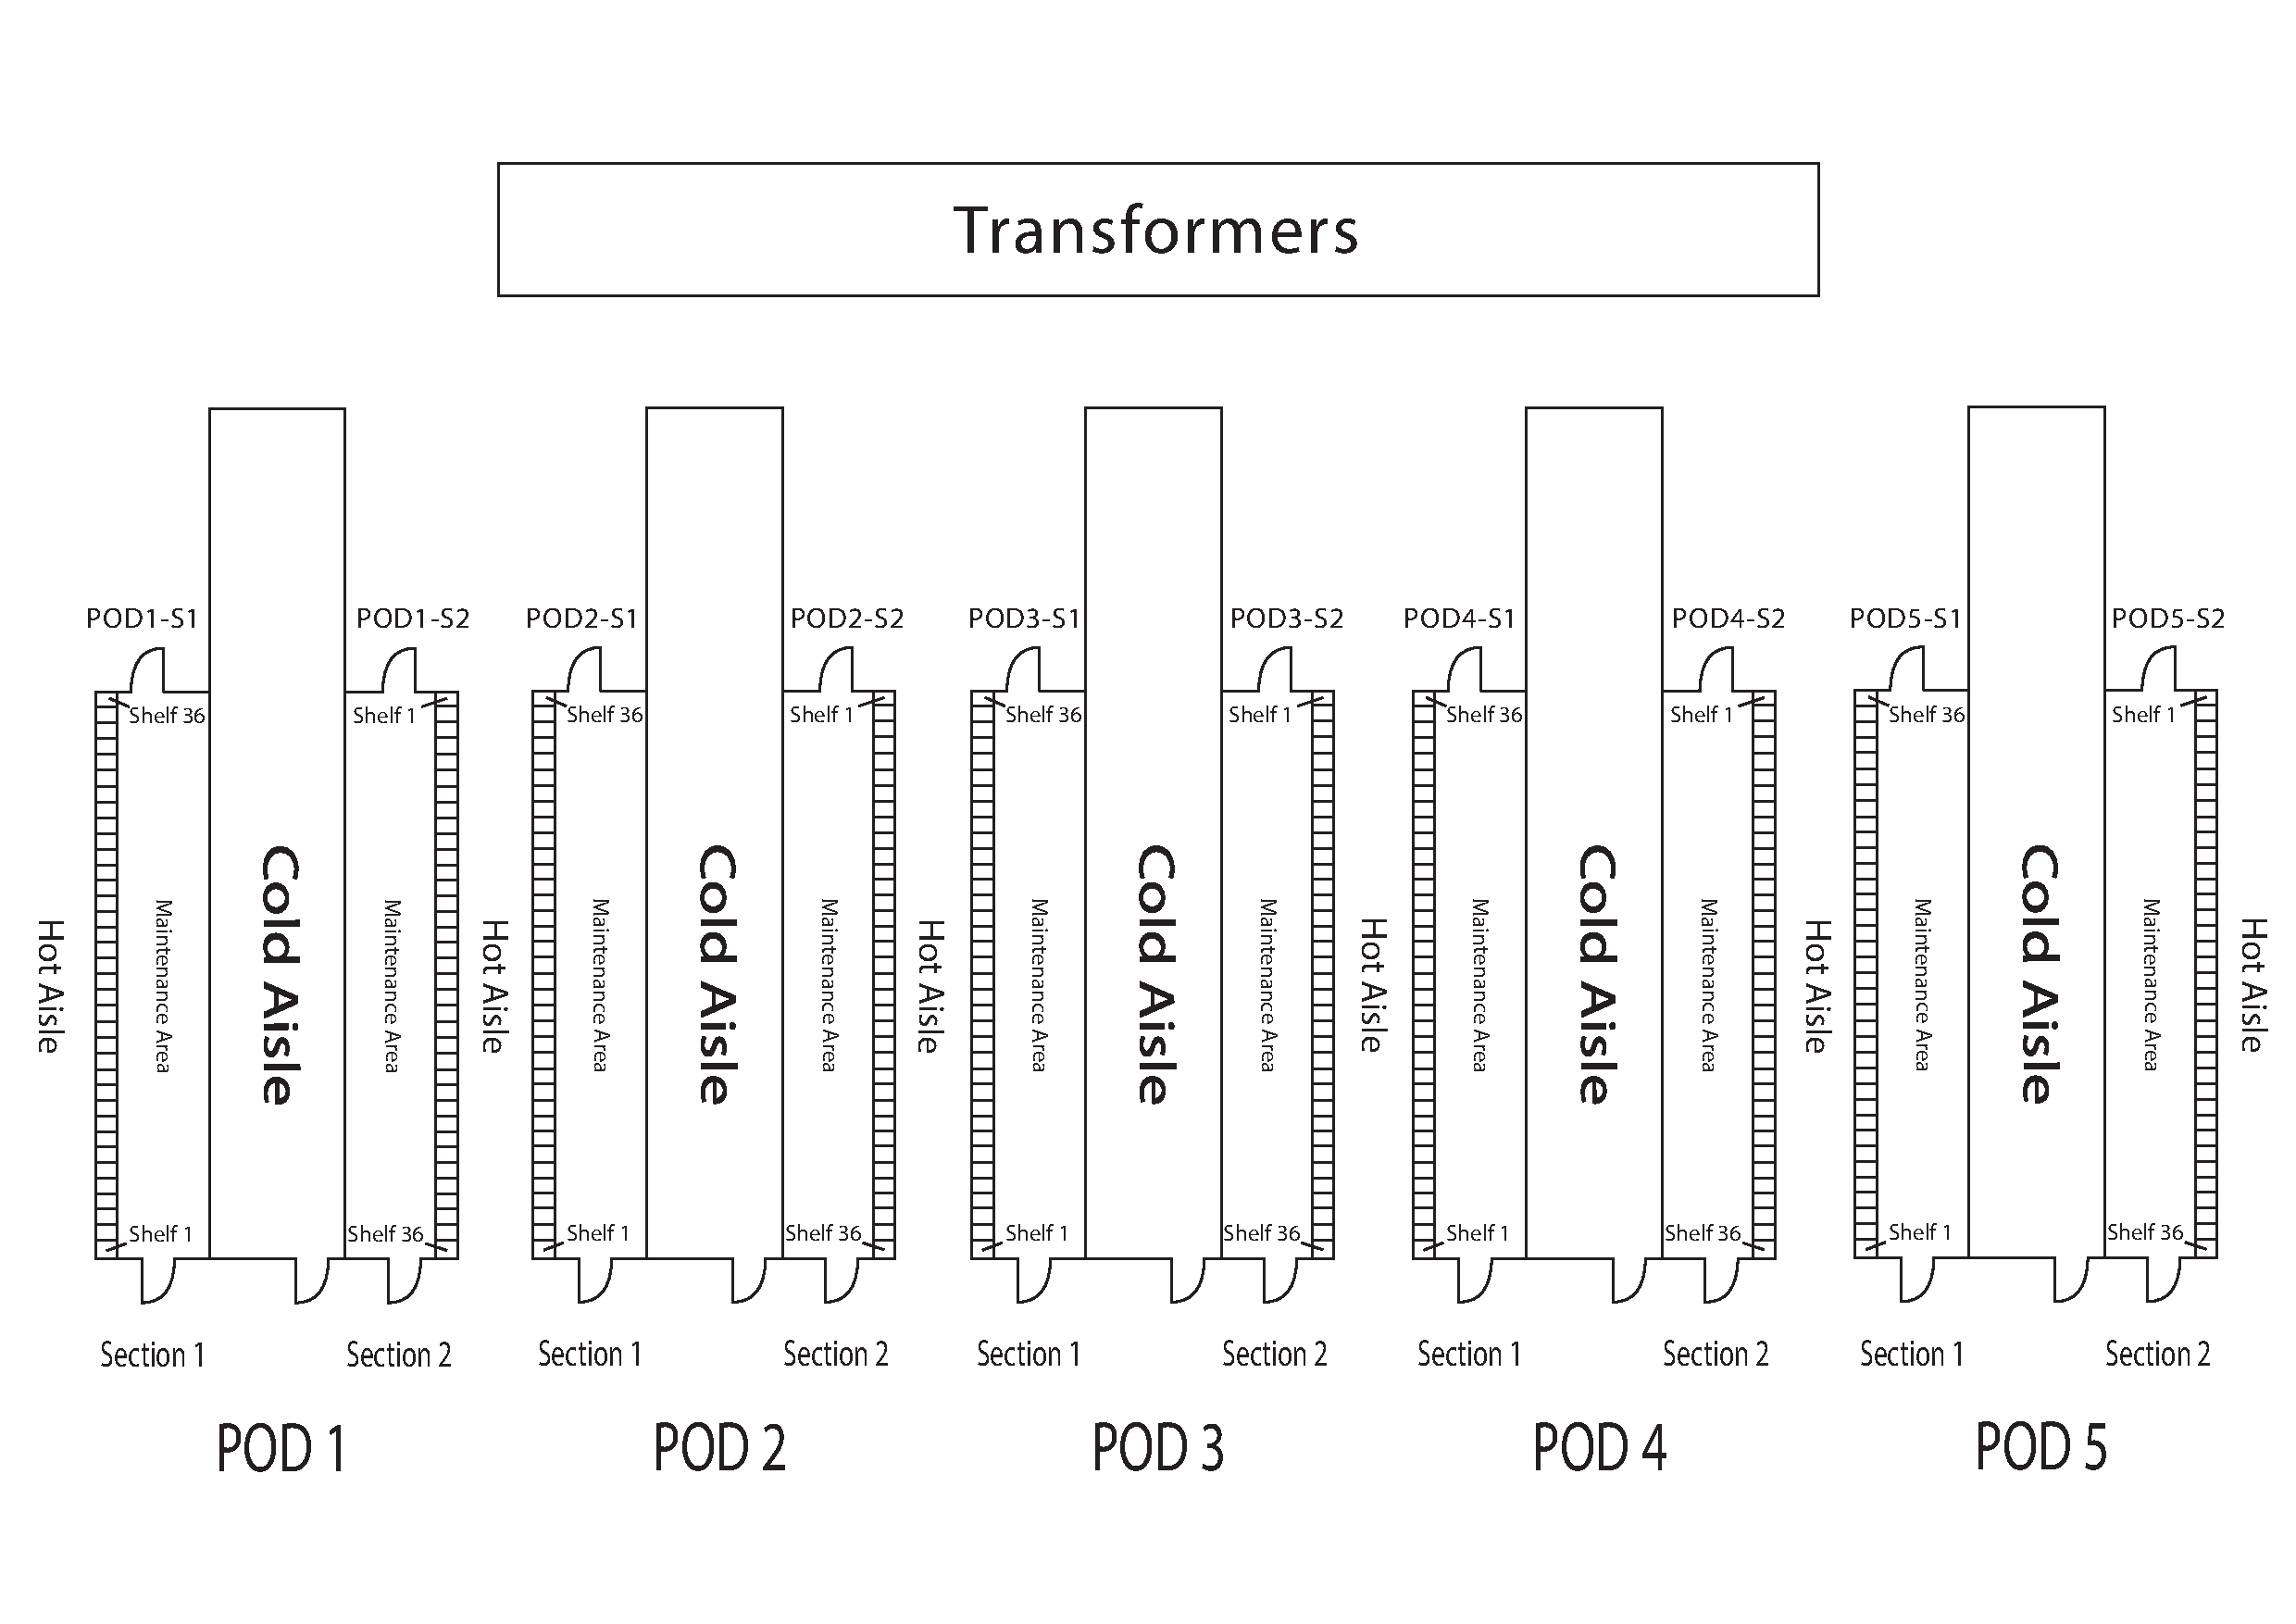
\includegraphics[page=1, angle=90, width=\linewidth]{layoutkardok.pdf} 

\newpage
\subsection{Functionality Mining Proxy} \label{toc:funktionsweiseminingproxy}
\includegraphics[width=\linewidth]{miningproxy}

\subsection{Network topology section} \label{toc:netzwerktopologieausschnitt}
\includegraphics[width=\linewidth]{networktopologykaz}

\newpage
\subsection{Summary of Investment} \label{toc:summaryofinvestment}
\includegraphics[width=0.7\linewidth]{summaryofinvestment}

\newpage
\subsection{CapEx} \label{toc:capex}
\includegraphics[width=\linewidth]{capex}

\newpage
\subsection{OpEx} \label{toc:opex}
\includegraphics[width=\linewidth]{opex}

\newpage
\subsection{S19Pro Assumptions} \label{toc:s19proassumptions}
\includegraphics[width=\linewidth]{minerassumptions}

\newpage
\subsection{Funding Worst-case scenario} \label{toc:finanzierungworstcase}
\includegraphics[width=\linewidth]{financingworstscenario}

\newpage
\subsection{Funding Most-Probable Scenario} \label{toc:finanzierungmostprobable}
\includegraphics[width=\linewidth]{financingprobablescenario}

\newpage
\subsection{Funding optimal scenario} \label{toc:finanzierungoptimal}
\includegraphics[width=\linewidth]{financingoptimalscenario}

\newpage
\subsection{Different runs of a Bitcoin price and hashrate Monte Carlo simulation. (06.11.2020)} \label{toc:montecarlosimulationvier}
\includegraphics[page=2, width=\linewidth]{monte-carlo.pdf}

\newpage
\subsection{Evolution of the Bitcoin price based on a Monte Carlo simulation (06.11.2020)} \label{toc:entwicklungbitcoinpreismc}
\includegraphics[page=1, width=\linewidth]{monte-carlo.pdf}

\newpage
\subsection{Evolution of Bitcoin's network hashrate based on Monte Carlo simulation. (06.11.2020)} \label{toc:entwicklunghashratemc}
\includegraphics[page=6, width=\linewidth]{monte-carlo.pdf}

\newpage
\subsection{Evolution of \ac{BTC} and \ac{USD} exchange rate starting from 06.11.2020}
\includegraphics[width=\linewidth]{btcusd}
\cite[Source:][]{tradingview2021btcusd}

\newpage
\section{Literature research} \label{toc:literaturrecherche}
\subsection{Literature taxonomy} \label{toc:literaturtaxonomie}

\begin{table}[H]
    \caption{Literature taxonomy}
    \label{tbl:literaturtaxonomie}
    \scriptsize
    \begin{tabularx}{\textwidth}[ht]{|X||X|X|X|X|}
		\hline
		\textbf{Charasteristic} & \multicolumn{4}{X|}{\textbf{Categories}} \\
		\hline\hline
			Focus & Research Outcomes & Research Methods & \checkmark \textbf{Theories} & \checkmark \textbf{Applications} \\
		\hline
			Goal & \checkmark \textbf{Integration} & Criticism & \checkmark \textbf{Central Issues} & \\
		\hline
			Organisation & Historical & \checkmark \textbf{Conceptual} & Methodological & \\
		\hline
			Perspective & \checkmark \textbf{Neutral Representiation} & Espousal of Position & & \\
		\hline  
			Audience & \checkmark \textbf{Specialised Scholars} & General Scholars & Practitioners and Politicians & General Public \\
		\hline
			Coverage & Exhaustive & Exhaustive and Selective & Representative & \checkmark \textbf{Central/Pivotal} \\
		\hline
    \end{tabularx}
    \cite[Source: Based on][]{cooper1988organizing}
\end{table}
  
\subsection{Results of the search process} \label{toc:suchprozessergebnis}

\begin{table}[H]
	\caption{Literature research}
	\label{tbl:suchprozessergebnis}
  	% \tiny
	\scriptsize
  	\begin{tabularx}{\textwidth}[ht]{|l|X|X|l|l|X|l|X|X|}
		\hline
		\textbf{No.} & \textbf{Title} & \textbf{Author} & \textbf{Year} & \textbf{Date} & \textbf{Search term} & \textbf{Search engine} & \textbf{Relevance} \\
		\hline\hline
		1 & How Elon Musk’s Twitter Activity Moves Cryptocurrency Markets & Ante & 2021 & 20.03.2021 & Bitcoin AND Tweet AND Elon AND Musk & Google Scholar & Influence of Social Media on the Bitcoin Price \\
		\hline
		2 & Business intelligence as a key strategy for development organizations & Azma \& Mostafapour & 2012 & 18.12.2020 & Loshin AND Business AND Intelligence & Google Scholar & Introduction BI \\
		\hline
		3 & Bitcoin as a transaction ledger: A composable treatment & Badertscher et al. & 2017 & 07.02.2021 & Bitcoin AND Ledger & Google Scholar & Poor predictability of BTC rates \\
		\hline
		4 & Bitcoin mining technology & Bhaskar \& Chuen & 2015 & 07.02.2021 & Bitcoin AND Cloud AND Mining & Google Scholar & Mining Pools, Cloud Mining, Hardware, Blockchain \\
		\hline
		5 & A comparative study of data analysis techniques & Bihani \& Patil & 2014 & 23.03.2021 & Business AND Analytics & Google Scholar & Types of Business Analytics \\
		\hline
		6 & Bitcoin Intelligence–Business Intelligence meets Crypto Currency & Boto{\c{s}} & 2017 & 06.02.2021 & Mining AND Cryptocurrency AND Business AND Intelligence & Google Scholar & BI and Cryptocurrencies \\
		\hline
		7 & Business intelligence strategy & Boyer et al. & 2010 &  & \textit{Buch im Besitz des Autors} & & BI Basics \\
		\hline
		8 & Modeling and Simulation of the Economics of Mining in the Bitcoin Market & Cocco \& Marchesi & 2016 & 05.04.2021 & Monte AND Carlo AND Simulation AND Bitcoin & Google Scholar & Use of Monte Carlo simulations \\
		\hline
	\end{tabularx}
\end{table}

\begin{table}[H]
	\scriptsize
  	\begin{tabularx}{\textwidth}[ht]{|l|X|X|l|l|X|l|X|X|}
		\hline
		\textbf{No.} & \textbf{Title} & \textbf{Author} & \textbf{Year} & \textbf{Date} & \textbf{Search term} & \textbf{Search engine} & \textbf{Relevance} \\
		\hline\hline
		9 & Optimizing sha256 in bitcoin mining & Courtois \& Grajek & 2014 & 06.02.2021 & Mining AND Cryptocurrency AND Optimization & Google Scholar &  \\
		\hline
		10 & From chaining blocks to breaking even: A study on the profitability of bitcoin mining from 2012 to 2016 & Derks et al. & 2018 & 07.02.2021 & Bitcoin AND Mining AND Venture & Google Scholar & Value and cost flows, cash flow, mining hardware \\
		\hline
		11 & What is business intelligence? & Foley, Guillemette & 2010 & 18.12.2020 & ((Business AND Intelligence) OR BI) AND Costs & Google Scholar & History, definition BI, BI process components \\
		\hline
		12 & Disrupting industries with blockchain: The industry, venture capital funding, and regional distribution of blockchain ventures & Friedlmaier et al. & 2017 & 07.02.2021 & Bitcoin AND Mining AND Venture & Google Scholar & Share of mining companies in startups \\
		\hline
		13 & Blockchain meets cloud computing: a survey & Gai et al. & 2020 & 06.02.2021 & Crypto AND Mining AND Optimization AND Hardware & Google Scholar & Cloud Mining \\
		\hline
		14 & Fallstudien als Forschungsmethode: Pl{\"a}doyer f{\"u}r einen Methodenpluralismus in der deutschen betriebswirtschaftlichen Forschung & Göthlich & 2003 & 11.03.2021 & \textit{Vorwärtssuche basierend auf Wilde \& Hess} &  & Methodology Case studies \\
		\hline
		15 & Demystifying crypto-mining: Analysis and optimizations of memory-hard pow algorithms & Han et al. & 2019 & 06.02.2021 & Mining AND Cryptocurrency AND Optimization & IEEExplore & Consensus algorithms \\
		\hline
		16 & Capturing value from big data--a taxonomy of data-driven business models used by start-up firms & Hartmann et al. & 2016 & 18.12.2020 & Data AND Driven AND Business & EBSCO & Data model, Key data, Key activities, Value proposition \\
		\hline
		17 & Assessing benefits of business intelligence systems--a case study & Ho{\v{c}}evar \& Jakli{\v{c}} & 2010 & 18.12.2020 & ((Business AND Intelligence) OR BI) AND Costs & Google Scholar & Added value BI, advantages through BI \\
		\hline
		18 & Business intelligence and implementation in a small enterprise & Horakova \& Skalska & 2013 & 18.12.2020 & ((Business AND Intelligence) OR BI) AND Implementation & Google Scholar & Stakeholders, added value, introduction of BI \\
		\hline
		19 & Data quality & Huh et al. & 1990 & 26.03.2021 & Data AND Quality & Google Scholar & Quality criteria for data \\
		\hline
  	\end{tabularx}
\end{table}

\begin{table}[H]
	\scriptsize
  	\begin{tabularx}{\textwidth}[ht]{|l|X|X|l|l|X|l|X|X|}
		\hline
		\textbf{No.} & \textbf{Title} & \textbf{Author} & \textbf{Year} & \textbf{Date} & \textbf{Search term} & \textbf{Search engine} & \textbf{Relevance} \\
		\hline\hline
		20 & Bitcoin Network Mechanics: Forecasting the BTC Closing Price Using Vector Auto-Regression Models Based on Endogenous and Exogenous Feature Variables & Ibrahim et al. & 2020 & 30.03.2021 & Forecasting AND Bitcoin AND Price AND Regression & Google Scholar & Prediction models bitcoin price \\
		\hline
		21 & Business intelligence (BI) success and the role of BI capabilities & Isik et al. & 2011 & 18.12.2020 & ((Business AND Intelligence) OR BI) AND Risk & Google Scholar & BI in general \\
		\hline
		22 & Business intelligence: An analysis of the literature & Jourdan et al. & 2008 & 18.12.2020 & (Business AND Intelligence) OR BI & Google Scholar & Methodology and BI \\
		\hline
		23 & The fundamentals of business intelligence & Kasemsap & 2016 & 18.12.2020 & Loshin AND Business AND Intelligence & Google Scholar & ROI Hypothese, BI in general \\
		\hline
		24 & Big data and business intelligence: Debunking the myths & Kimble \& Milolidakis & 2015 & 26.03.2021 & Data AND In AND Business AND Intelligence & Google Scholar & Data types for BI \\
		\hline
		25 & Understanding Information System agility--the example of business intelligence & Knabke \& Olbrich & 2013 & 18.12.2020 & ((Business AND Intelligence) OR BI) AND Scrum & Google Scholar & Literature Review, Definition of Agility \\
		\hline
		26 & The economics of Bitcoin mining, or Bitcoin in the presence of adversaries & Kroll et al. & 2013 & 07.02.2021 & Bitcoin AND Mining & Google Scholar & Explanation of mining \\
		\hline
		27 & Blockchain-enabled data provenance in cloud datacenter reengineering & Li et al. & 2019 & 06.02.2021 & Crypto AND Mining AND Data AND Center & Google Scholar & Explanation of PoW \\
		\hline
		28 & Business intelligence: the savvy manager's guide & Loshin & 2012 &  & \textit{Buch im Besitz des Autors} &  & BI Basics \\
		\hline
		29 & Grundz{\"u}ge der Wirtschaftsinformatik & Mertens et al. & 2005 & & & & Definition Business Informatics \\
		\hline
		30 & A brief survey of cryptocurrency systems & Mukhopadhyay et al. & 2016 & 17.02.2021 & Mining AND Cryptocurrency & Google Scholar & BTC history \\
		\hline
		31 & Agile BI-The Future of BI. & Muntean \& Surcel & 2013 & 18.12.2020 & ((Business AND Intelligence) OR BI) AND Scrum & Google Scholar & BI process, Scrum as methodology \\
		\hline
		32 & Bitcoin: A peer-to-peer electronic cash system & Nakamoto & 2008 & 07.02.2021 & Bitcoin AND Whitepaper & Google Scholar & Bitcoin, Blockchain, Mining \\
		\hline
		33 & Cognition-driven decision support for business intelligence & Niu et al. & 2009 & 18.12.2020 & Business Intelligence OR BI & Google Scholar & BI process, OLAP, warehouses, analysis options \\
		\hline
		34 & Big data business intelligence in bank risk analysis & Rahman \& Iverson & 2015 & 18.12.2020 & ((Business AND Intelligence) OR BI) AND Risk & Google Scholar & IT Architecture Big Data \\
		\hline
		35 & Business justification with business intelligence & Ranjan & 2008 & 18.12.2020 & Loshin AND Business AND Intelligence & EBSCO & BI Definition and Components \\
		\hline
	\end{tabularx}
\end{table}

\begin{table}[H]
	\scriptsize
  	\begin{tabularx}{\textwidth}[ht]{|l|X|X|l|l|X|l|X|X|}
		\hline
		\textbf{No.} & \textbf{Title} & \textbf{Author} & \textbf{Year} & \textbf{Date} & \textbf{Search term} & \textbf{Search engine} & \textbf{Relevance} \\
		\hline\hline
		36 & Who's in and why? A typology of stakeholder analysis methods for natural resource management & Reed et al. & 2009 & 01.04.2021 & Stakeholder AND Analysis AND Business AND Intelligence & Google Scholar & Stakeholder analysis \\
		\hline
		37 & A stakeholder model of business intelligence & Simmers & 2004 & 11.03.2021 & Stakeholder AND Business AND Intelligence & Google Scholar & Stakeholder analysis \\
		\hline
		38 & The usefulness of ERP systems for effective management & Spathis \& Constantinides & 2003 & 22.03.2021 & ERP AND Systems AND Financial AND Accounting & Google Scholar & Overview ERP \\
		\hline
		39 & The evolution of bitcoin hardware & Taylor & 2017 & 06.02.2021 & Crypto AND Mining AND Optimization AND Hardware & IEEExplore & History of mining \\
		\hline
		40 & Key success factors to business intelligence solution implementation & Villamar\'{i}n \& Diaz Pinzon & 2017 & 18.12.2020 & Loshin AND Business AND Intelligence & Google Scholar & Role PM and Top Management in BI \\
		\hline
		41 & The current state of business intelligence & Watson \& Wixom & 2007 & 18.12.2020 & (Business AND Intelligence) OR BI & Google Scholar & BI Benefits, BI Success, History \\
		\hline
		42 & Methodenspektrum der Wirtschaftsinformatik & Wilde \& Hess & 2006 & 11.03.2021 & Methoden AND Wirtschaftsinformatik & Google Scholar & Overview methodologies \\
		\hline
		43 & Forschungsmethoden der Wirtschaftsinformatik & Wilde \& Hess & 2007 & 11.03.2021 & Methoden AND Wirtschaftsinformatik & Google Scholar & Overview methodologies \\
		\hline
		44 & The business value of business intelligence & Williams \& Williams & 2003 & 18.12.2020 & ((Business AND Intelligence) OR BI) AND Project AND Management & Google Scholar & Added value BI \\
		\hline
		45 & Extreme datacenter specialization for planet-scale computing: Asic clouds & Xie et al. & 2018 & 06.02.2021 & Crypto AND Mining AND Data AND Center & Google Scholar & ASIC Clouds \\
		\hline
		46 & Critical success factors for business intelligence systems & Yeoh \& Koronius & 2010 & 18.12.2020 & (Business Intelligence OR BI) AND Project AND Management & Google Scholar & Definition BI \\
		\hline
		47 & Managing the implementation of business intelligence systems: a critical success factors framework & Yeoh et al. & 2008 & 18.12.2020 & (Business Intelligence OR BI) AND Project AND Management & Google Scholar & Requirements BI and IS \\
		\hline
	\end{tabularx}
\end{table}

\newpage
Internet sources:

\begin{table}[H]
	\scriptsize
  	\begin{tabularx}{\textwidth}[ht]{|l|X|X|l|l|X|l|X|X|}
		\hline
		\textbf{No.} & \textbf{Title} & \textbf{Author} & \textbf{Year} & \textbf{Date} & \textbf{Search term} & \textbf{Search engine} & \textbf{Relevance} \\
		\hline\hline
		48 & Configure privileged API access for Antminer & Awesome Miner & & 22.03.2021 & & & Mining Hardware API \\
		\hline
		49 & Bitcoin Price in USD vs. Tweets historical chart & bitinfocharts.com & 20.03.2021 & 20.03.2021 & & & Influence of Social Media on the Bitcoin Price \\
		\hline
		50 & S19 Pro Server Installation Guide & Bitmain & 01.04.2020 & 22.03.2021 & & & Mining hardware functionality \\
		\hline
		51 & Bitcoin Developer APIs & blockchain.com & 20.03.2021 & 20.03.2021 & & & Blockchain interface \\
		\hline
		52 & Total Hash Rate (TH/s) & blockchain.com & 20.03.2021 & 20.03.2021 & & & Hashrate von Bitcoin \\
		\hline
		53 & Pool Distribution (calulate by blocks) & btc.com & 07.02.2021 & 07.02.2021 & Große AND Bitcoin AND Miner & Google & Hashrate distribution \\
		\hline
		54 & getdifficulty & developer.bitcoin.org & 20.03.2021 & 20.03.2021 & & & Blockchain interface \\
		\hline
		55 & getrawmempool & developer.bitcoin.org & 20.03.2021 & 20.03.2021 & & & Blockchain interface \\
		\hline
		56 & What is a data warehouse? & Google Cloud & & 12.04.2021 & Google AND Cloud AND Data AND Warehouse & Google & Google Cloud products \\
		\hline
		57 & Google Cloud Scheduler & Google Cloud Scheduler & & 14.04.2021 & Google AND Cloud AND Cronjobs & Google & Google Cloud products \\
		\hline
		58 & S19 Pro Specifications & Jocelyn & 27.02.2020 & 23.02.2021 & S19 Pro AND Miner AND Spec & Google & Power consumption S19 Pro Miner \\
		\hline
		59 & Bitcoin-Halving abgeschlossen: Ab jetzt nur noch 6,25 BTC pro Block & Klee & 11.05.2020 & 19.02.2021 & Bitcoin AND Halving & Google & Current Block Reward \\
		\hline
		60 & Der unersättliche Stromfresser: Bitcoin & Rooks & 16.02.2021 & 19.02.2021 & Mining AND Stromverbrauch & Google & Power consumption Mining \\
		\hline
		61 & How Elon Musk Moves The Price Of Bitcoin With His Twitter Activity & Shelvin & 21.02.2021 & 20.03.2021 & Bitcoin AND Tweet AND Elon AND Musk & Google & Influence of Social Media on the Bitcoin Price \\
		\hline
		62 & BTCUSD & tradingview.com & 29.04.2021 & 29.04.2021 & Bitcoin AND Price AND Charts & Google & Bitcoin price evolution \\
		\hline
		63 & The top 10 blockchain trends for 2021 & Wiesflecker & 26.02.2021 & 21.04.2021 & Blockchain AND Technology AND Trends & Google & Trends in blockchain technology \\
		\hline
		64 & Pricing & World Weather Online & 20.03.2021 & 20.03.2021 & & & Weather data interface \\
		\hline
		65 & Weather API & World Weather Online & 20.03.2021 & 20.03.2021 & & & Weather data interface \\
		\hline
	\end{tabularx}
\end{table}

\subsection{Concept matrix} \label{toc:konzeptmatrix}

\begin{table}[H]
    \caption{Concept matrix}
	\label{tbl:konzeptmatrix}
	\scriptsize
    \begin{tabularx}{\textwidth}[ht]{|l|X|X|X|X|X|X|X|X|}
		\hline
		\textbf{Source no. according to table \ref{tbl:suchprozessergebnis}} & \multicolumn{6}{c|}{\textbf{Concepts}} \\
		& {Business Intelligence} & {Blockchain \& Mining} & {Stakeholder analysis} & {(Big) Data} & {Cloud} & {Methodology} \\
		\hline\hline
		1 &  & \centering \checkmark &  & \centering \checkmark &  & \tabularnewline \hline
		2 & \centering \checkmark &  &  &  &  & \tabularnewline \hline
		3 &  & \centering \checkmark &  &  &  & \tabularnewline \hline
		4 &  & \centering \checkmark &  &  &  & \tabularnewline \hline
		5 &  &  &  & \centering \checkmark &  & \tabularnewline \hline
		6 & \centering \checkmark & \centering \checkmark &  &  &  & \tabularnewline \hline
		7 & \centering \checkmark &  &  &  &  & \tabularnewline \hline
		8 &  & \centering \checkmark &  & \centering \checkmark &  & \tabularnewline \hline
		9 &  & \centering \checkmark &  &  &  & \tabularnewline \hline
		10 &  & \centering \checkmark &  & \centering \checkmark &  & \tabularnewline \hline
		11 &  & \centering \checkmark &  &  &  & \tabularnewline \hline
		12 &  & \centering \checkmark &  &  &  & \tabularnewline \hline
		13 &  & \centering \checkmark &  &  & \centering \checkmark & \tabularnewline \hline
		14 &  &  &  &  &  & \centering \checkmark \tabularnewline \hline
		15 & \centering \checkmark &  &  &  &  & \tabularnewline \hline
		16 &  &  &  & \centering \checkmark &  & \centering \checkmark \tabularnewline \hline
		17 & \centering \checkmark &  &  &  &  & \tabularnewline \hline
		18 & \centering \checkmark &  &  &  &  & \tabularnewline \hline
		19 &  &  &  & \centering \checkmark &  & \tabularnewline \hline
		20 &  & \centering \checkmark &  & \centering \checkmark &  & \tabularnewline \hline
		21 & \centering \checkmark &  &  &  &  & \tabularnewline \hline
		22 & \centering \checkmark &  &  &  &  & \centering \checkmark \tabularnewline \hline
		23 & \centering \checkmark &  &  &  &  & \tabularnewline \hline
		24 & \centering \checkmark &  &  & \centering \checkmark &  & \tabularnewline \hline
		25 & \centering \checkmark &  &  &  &  & \tabularnewline \hline
		26 &  & \centering \checkmark &  & \centering \checkmark &  & \tabularnewline \hline
		27 &  & \centering \checkmark &  &  & \centering \checkmark & \tabularnewline \hline
		28 & \centering \checkmark &  &  &  &  & \tabularnewline \hline
		29 &  &  &  &  &  & \centering \checkmark \tabularnewline \hline
		30 &  & \centering \checkmark &  &  &  & \tabularnewline \hline
		31 & \centering \checkmark &  &  &  &  & \tabularnewline \hline
		32 &  & \centering \checkmark &  &  &  & \tabularnewline \hline
		33 & \centering \checkmark &  &  &  &  & \tabularnewline \hline
		34 & \centering \checkmark &  &  & \centering \checkmark &  & \tabularnewline \hline
		35 & \centering \checkmark &  &  &  &  & \tabularnewline \hline
		36 & \centering \checkmark &  & \centering \checkmark &  &  & \tabularnewline \hline
		37 & \centering \checkmark &  & \centering \checkmark &  &  & \tabularnewline \hline
		38 & \centering \checkmark &  &  &  &  & \tabularnewline \hline
		39 &  & \centering \checkmark &  &  &  & \tabularnewline \hline
		40 & \centering \checkmark &  &  &  &  & \tabularnewline \hline
		41 & \centering \checkmark &  &  &  &  & \tabularnewline \hline
		42 &  &  &  &  &  & \centering \checkmark \tabularnewline \hline
		43 &  &  &  &  &  & \centering \checkmark \tabularnewline \hline
		44 & \centering \checkmark &  &  &  &  & \tabularnewline \hline
		45 &  & \centering \checkmark &  &  & \centering \checkmark & \tabularnewline \hline
		46 & \centering \checkmark &  &  &  &  & \tabularnewline \hline
		47 & \centering \checkmark &  &  &  &  & \tabularnewline \hline
		48 &  & \centering \checkmark &  &  &  & \tabularnewline \hline
		49 &  & \centering \checkmark &  &  &  & \tabularnewline \hline
		50 &  & \centering \checkmark &  &  &  & \tabularnewline \hline
	\end{tabularx}
\end{table}

\begin{table}[H]
	\scriptsize
    \begin{tabularx}{\textwidth}[ht]{|l|X|X|X|X|X|X|X|X|}
		\hline
		\textbf{Source no. according to table \ref{tbl:suchprozessergebnis}} & \multicolumn{6}{c|}{\textbf{Concepts}} \\
		& {Business Intelligence} & {Blockchain \& Mining} & {Stakeholder analysis} & {(Big) Data} & {Cloud} & {Methodology} \\
		\hline\hline
		51 &  & \centering \checkmark &  & \centering \checkmark &  & \tabularnewline \hline
		52 &  & \centering \checkmark &  & \centering \checkmark &  & \tabularnewline \hline
		53 &  & \centering \checkmark &  &  &  & \tabularnewline \hline
		54 &  & \centering \checkmark &  & \centering \checkmark &  & \tabularnewline \hline
		55 &  & \centering \checkmark &  & \centering \checkmark &  & \tabularnewline \hline
		56 &  &  &  &  & \centering \checkmark & \tabularnewline \hline
		57 &  &  &  &  & \centering \checkmark & \tabularnewline \hline
		58 &  & \centering \checkmark &  &  &  & \tabularnewline \hline
		59 &  & \centering \checkmark &  &  &  & \tabularnewline \hline
		60 &  & \centering \checkmark &  &  &  & \tabularnewline \hline
		61 &  & \centering \checkmark &  & \centering \checkmark &  & \tabularnewline \hline
		62 &  & \centering \checkmark &  &  &  & \tabularnewline \hline
		63 &  & \centering \checkmark &  &  &  & \tabularnewline \hline
		64 &  &  &  & \centering \checkmark &  & \tabularnewline \hline
		65 &  &  &  & \centering \checkmark &  & \tabularnewline \hline
	\end{tabularx}
	\cite[Source: Based on][]{webster2002analyzing}
\end{table}